\chapter{Tecnologías}

\section{Node.js}

Node.js es un entorno de ejecución para JavaScript construido con el motor de JavaScript
V8 de Chrome. En este proyecto se ha utilizado para elaborar el servidor de la aplicación.\\

Node.js tiene una característica que lo diferencia del resto de posibilidades para implementar 
el servidor y es que utiliza un modelo de operaciones E/S sin bloqueo y orientado a eventos 
asícronos. Esto nos ofrece la la posibilidad para que cuando se detecte una conexión se atienda
pero el resto del tiempo estará inactivo. Con este nuevo modelo conseguimos servidores altamente 
escalables de una manera muy sencilla, rápida y eficiente.\\

\begin{figure}[H]
	\centering
	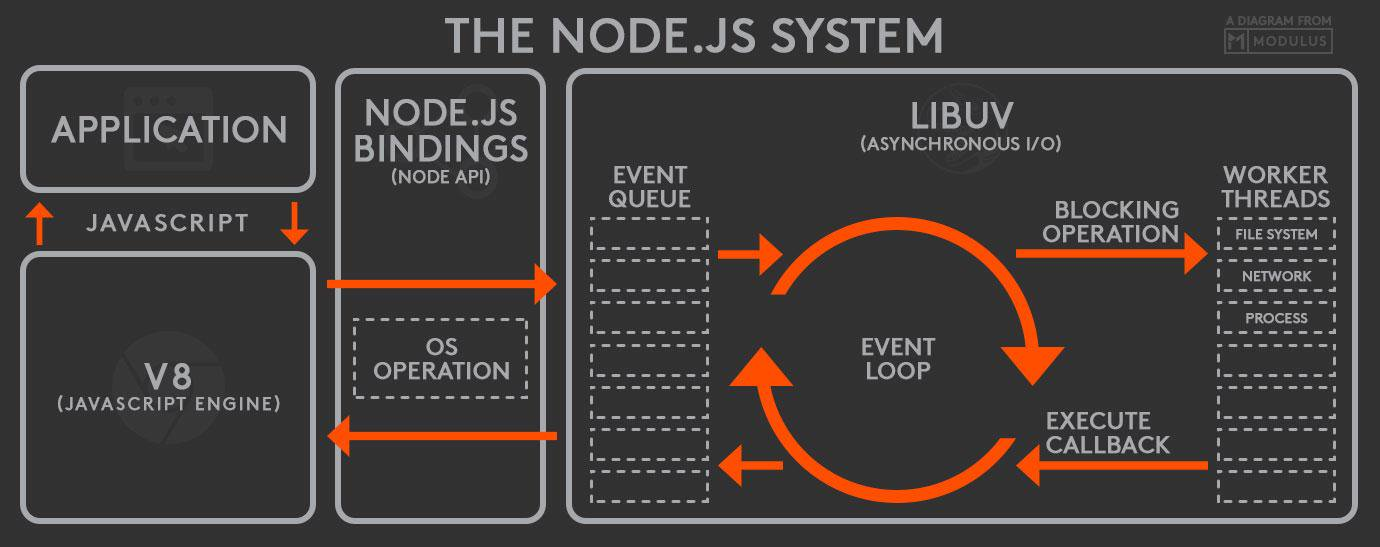
\includegraphics[scale=0.25]{imagenes/nodejs_system.jpg}
	\caption{Sistema de Nodejs \label{fig:figura1}}
\end{figure}

Este diseño contrasta directamente con el modelo con el modelo de concurrencia más común hoy en 
día en el que se usan hilos del Sistema Operativo. Las operaciones en red basadas en este modelo
son relativamente ineficientes además de complejas en su uso. Cabe mencionar que, aunque Node.js 
no utilice hilos del Sistema Operativo implique que no podamos aprovechar los múltiples cores
de nuestro sistema.\\

Otro punto a favor de Node.js es que no tendremos que preocuparnos por la posibilidad de un 
bloqueo en el proceso debido a que no existe dicha posibilidad por la naturaleza de dicha 
tecnología, la cual está basada en un bucle de eventos.

\section{MongoDB}

MongoDB es un sistema de base de datos multiplataforma y orientado a documentos de esquema libre.
Esto quiere decir que cada entrada puede tener un esquema de datos diferente al anterior, por
lo que podemos tener entradas que difieran en el número de atributos entre sí.\\

Debido a esta característica los datos no son guardados en registros, como en las bases SQL, 
sino que se guardan en documentos. Estos documentos son del tipo BSON, que es una representación
binaria de los archivos JSON.\\

Esta tecnología ha sido escrita en C++, por lo que está en contacto con el \textit{bare metal}. Esto
último es realmente importante ya que le permite optimizar los recursos y acceder a ellos de una 
manera extremadamente eficiente, con lo que consigue una velocidad muy alta en todas sus operaciones.\\

Cabe mencionar que MongoDB es una plataforma completamente distribuida, lo que nos proporciona 
un nuevo nivel de escalabilidad y disponibilidad. Esto quiere decir que a medida que nuestro desarrollo
crezca tanto en volumen de datos como en rendimiento MongoDB se escala automáticamente sin tiempos
de caída y sin cambios en nuestra aplicación.\\

Por último, cabe mencionar que la licencia de esta tecnología es GNU AGPL 3.0, por lo que se trata de un software de licencia
libre.

% insertar mongodb schema

\section{Vagrant}

Vagrant es una herramienta para construir y administrar entornos de máquinas virtuales de una 
manera sencilla. Debido a que está diseñado para ser sencillo de utilizar y a que se centra en 
la automatización hace que utilicemos el menor tiempo posible en la preparación del entorno virtual
que necesitamos para comenzar a trabajar.\\

Nos proporciona un entorno muy rápido y simple de configurar, reproducible y portable utilizando
tecnología puntera en el sector de la virtualización como puede ser VirtualBox, VMWare, AWS, Docker...\\

Una enorme ventaja que aporta Vagrant al desarrollo es la posibilidad de aislar toda la configuración
del entorno y todas sus dependencias. Además, no tiene que deshacerse de las herramientras de trabajo
a las que está acostumbrado, pues realmente se sigue trabajando en el mismo entorno. 
De esta manera se consigue un desarrollo más eficiente y con mínimas pérdidas de tiempo, garantizando 
de manera directa una eficiencia en la gestión de los recursos humanos empleados.\\

% insertar vagrant advantages


\section{Ansible}

Ansible es un software que se ha diseñado explícitamente para automatizar acciones y
conseguir una mayor productividad. De esta manera, se libera al equipo de tareas costosas
y que siempre siguen el mismo proceso.\\

Ansible está categorizado bajo el nombre de \textbf{herramineta de orquestación} debido a 
las funciones que realiza. Se encarga de manejar nodos a través de SSH habiendo recibido
una entrada por parte del usuario. De esta manera, se le entrega una entrada muy sencilla
y comprensible para la lectura del ser humano, que posteriormente es analizada y transformada
en una serie de tareas hacia los nodos, consiguiendo quedar completamente configurados de una
manera muy rápida y sencilla.\\

% insertar ansible workflow

Es la herramienta de automatización de código libre más potente actualmente y esto es reflejado
en las estadísticas de GitHub del proyecto. Además, la comunidad está implicada muy directamente
en el desarrollo de esta herramienta ya que cuenta con más de 2.400 personas que han desarrollado
uno o varios módulos para mejorarla.



